\documentclass[aspectratio=169]{beamer}

%\usefonttheme[onlymath]{serif} %%%%%%%%%

\usetheme{NRLpresentationGWU}

\RequirePackage{NRLcolors}


%\titlegraphic{\includegraphics[width=0.9\textwidth]{$HOME/Documents/TAVEX/gmt/TAVEX-overview-3}}% optional


\usepackage{cite}
\usepackage{amsmath,amssymb,amsfonts}
\usepackage{algorithmic}
\usepackage{graphicx}
\usepackage{textcomp}
\usepackage{bm}
\usepackage{upgreek}

\usepackage[retainorgcmds]{IEEEtrantools}

%\usepackage{hyperref}

\usepackage{hhline}





\setlength{\fboxsep}{3pt}
\setlength{\fboxrule}{2pt}



%\graphicspath{ {C:/Users/Paul/Documents/PhD/Dissertation/Documentation/Figures/} }
\graphicspath{ {../Figures/} }


\DeclareMathOperator*{\argmin}{arg\,min}
\DeclareMathOperator*{\argmax}{arg\,max}

\DeclareMathOperator{\xrm}{\mathrm{x}}
\DeclareMathOperator{\Xrm}{\mathrm{X}}
\DeclareMathOperator{\yrm}{\mathrm{y}}
\DeclareMathOperator{\Yrm}{\mathrm{Y}}
\DeclareMathOperator{\Drm}{\mathrm{D}}
\DeclareMathOperator{\nrm}{\mathrm{n}}
\DeclareMathOperator{\nbarrm}{\bar{\mathrm{n}}}
\DeclareMathOperator{\zrm}{\mathrm{z}}

\DeclareMathOperator{\Prm}{\mathrm{P}}
\DeclareMathOperator{\prm}{\mathrm{p}}
\DeclareMathOperator{\Erm}{\mathrm{E}}
\DeclareMathOperator{\Crm}{\mathrm{C}}

\DeclareMathOperator{\Xcal}{\mathcal{X}}
\DeclareMathOperator{\Ycal}{\mathcal{Y}}
\DeclareMathOperator{\Dcal}{\mathcal{D}}
\DeclareMathOperator{\Ncal}{\mathcal{N}}
\DeclareMathOperator{\Zcal}{\mathcal{Z}}
\DeclareMathOperator{\Hcal}{\mathcal{H}}
\DeclareMathOperator{\Fcal}{\mathcal{F}}
\DeclareMathOperator{\Rcal}{\mathcal{R}}
\DeclareMathOperator{\Mcal}{\mathcal{M}}
\DeclareMathOperator{\Scal}{\mathcal{S}}
\DeclareMathOperator{\Pcal}{\mathcal{P}}
\DeclareMathOperator{\Lcal}{\mathcal{L}}

\DeclareMathOperator{\Rbb}{\mathbb{R}}
\DeclareMathOperator{\Nbb}{\mathbb{N}}
\DeclareMathOperator{\Zbb}{\mathbb{Z}}

\DeclareMathOperator{\Dir}{\mathrm{Dir}}
\DeclareMathOperator{\DM}{\mathrm{DM}}
\DeclareMathOperator{\Multi}{\mathrm{Multi}}
\DeclareMathOperator{\DP}{\mathrm{DP}}
\DeclareMathOperator{\DMP}{\mathrm{DMP}}


\newcommand\independent{\protect\mathpalette{\protect\independenT}{\perp}}
\def\independenT#1#2{\mathrel{\rlap{$#1#2$}\mkern2mu{#1#2}}}




\title{Bayesian Learning for Classification using a Uniform Dirichlet Prior}
%\subtitle{Work Supported by the U.S. Office of Naval Research}% optional

\author[Rademacher \& Doroslova\v{c}ki]{Paul Rademacher\inst{1} \and Milo\v{s} Doroslova\v{c}ki\inst{2}}
\institute[NRL,~GWU] 
{
  \inst{1}
  U.S. Naval Research Laboratory\\Radar Division
  \and
  \inst{2}
  The George Washington University\\Department of Electrical and Computer Engineering
}


\date{November 13, 2019}


%\NRLcredit{Work Supported by the U.S. Office of Naval Research}% optional
%\NRLmark{FOR OFFICIAL USE ONLY}% optional
%\NRLpatents{Example Patents\\7,749,438 and 7,754,145}% optional

\NRLdist{DISTRIBUTION A. Approved for public release: distribution unlimited.}
%\NRLfoot{DISTRIBUTION A. Approved for public release: distribution unlimited.}


\begin{document}


\begin{frame}
\titlepage
\end{frame}


\begin{frame}
\frametitle{Introduction}
\framesubtitle{Part I}

Bayesian approaches to machine learning attempt to make better decisions by exploiting \emph{prior knowledge} regarding the data-generating distribution:

\vspace{1em}

\begin{columns}[T]

\begin{column}{.5\linewidth}

\centering
\large \textbf{\underline{Informative}} \normalsize
\vspace{0.5em}
\begin{itemize}
\item If the prior is localized around the true data-generating model, low-risk decisions can be made even with limited training data
\item Priors that assign low weighting to the true model may not be able to realize satisfactory performance 
\end{itemize}


\end{column}

\vrule

\begin{column}{.5\linewidth}

\centering
\large \textbf{\underline{Non-Informative}} \normalsize
\vspace{0.5em}
\begin{itemize}
\item Learners designed with approximately uniform priors will not perform as well as those made with well-selected informative priors
\item Avoid high risk inherent to learners made by mismatched informative priors
\end{itemize}



\end{column}

\end{columns}

\end{frame}




\begin{frame}
\frametitle{Introduction}
\framesubtitle{Part II}

\begin{itemize}
\item Often, priors are termed non-informative as long as they are approximately uniform over their \underline{limited support}. For example, a parametric regression function might use a high covariance Gaussian vector prior to characterize a subset of probability distributions
\vspace{0.5em}
\item The uniform Dirichlet distribution is unique in that it has \underline{full support} over the space of data-generating distributions and is thus truly non-informative
\vspace{0.5em}
\item Additionally, it is a \emph{conjugate prior} for independent, identically distributed observations and leads to a closed-form model posterior distribution

\end{itemize}

\end{frame}



\section{Objective and Bayesian Setup}


\begin{frame}
\frametitle{Data Model}

\begin{description}
\item[Observable random element:] $\xrm \in \Xcal$
\item[Unobservable random element:] $\yrm \in \Ycal$
\item[Observable training data:] $\Drm \in \Dcal = \{\Ycal \times \Xcal\}^N$
\end{description}

\vspace{0.5em}

Independently, identically distributed according to an \underline{unknown} probability mass function (PMF) 
\begin{equation*}
\theta \in \Theta = \left\{ \theta \in {\Rbb_{\geq 0}}^{\Ycal \times \Xcal}: \sum_{y \in \Ycal} \sum_{x \in \Xcal} \theta(y,x) = 1 \right\} \ ,
\end{equation*}
such that $\Prm_{\yrm,\xrm | \uptheta}(y,x | \theta) = \Prm_{\Drm_n | \uptheta}(y,x | \theta) = \theta(y,x)$.

\hrulefill

\vspace{0.5em}
\textit{Alternate Notation}: $\theta \Leftrightarrow \big( \theta',\tilde{\theta} \big)$
\begin{itemize}
\item Marginal model $\theta' \equiv \sum_{y \in \Ycal} \theta(y,\cdot) = \Prm_{\xrm | \uptheta}$ over the set $\Xcal$ 
\item Conditional models $\tilde{\theta}(\xrm) \equiv \theta(\cdot,\xrm) / \theta'(x) = \Prm_{\yrm | \xrm,\uptheta}$ over the set $\Ycal$
\end{itemize}

\end{frame}




\begin{frame}
\frametitle{Sufficient Statistic}


\begin{columns}[c]


\begin{column}{.5\linewidth}

Training data PMF:
\begin{IEEEeqnarray}{C}
\Prm_{\Drm | \uptheta}(D | \theta) = \prod_{y \in \Ycal} \prod_{x \in \Xcal} \theta(y,x)^{\bar{N}(y,x;D)} \nonumber 
\end{IEEEeqnarray}
is expressed via $\bar{N}(y,x;D) = \sum_{n=1}^N \delta\big[ (y,x),D_n \big]$, with range 
\begin{equation*}
\bar{\Ncal} = \left\{ \bar{n} \in {\Zbb_{\geq 0}}^{\Ycal \times \Xcal}: \sum_{y \in \Ycal} \sum_{x \in \Xcal} \bar{n}(y,x) = N \right\}
\end{equation*}

\end{column}

\vrule
\hspace{0.5ex}
\begin{column}{.5\linewidth}

\begin{itemize}
\item Empirical count $\bar{N}(\Drm)$ is a \emph{sufficient statistic} for the model $\uptheta$
\vspace{0.5em}
\item $|\bar{\Ncal}| = \binom{N+|\Ycal||\Xcal|-1}{|\Ycal||\Xcal|-1} \leq |\Dcal|$  
\vspace{0.5em}
\begin{itemize}
\item [$\Rightarrow$] \large \textbf{Efficient Transform} \normalsize
\end{itemize}
\end{itemize}

\vspace{-1em}
 
\Large
\begin{equation*} 
\Downarrow \quad \Downarrow
\end{equation*}
\normalsize
\vspace{-1.0em}
\begin{block}{Compact Representation}
\centering
\textbf{Express distributions using new \\random process $\nbarrm \equiv \bar{N}(\Drm) \in \bar{\Ncal}$}
\end{block}

\end{column}

\end{columns}

\end{frame}





\begin{frame}
\frametitle{Objective}

\begin{columns}[c]


\begin{column}{.5\linewidth}

\vspace{2em}

\begin{block}{Design Metric}
User-selected function $\Lcal: \Ycal \times \Ycal \mapsto \Rbb_{\geq 0}$. Most commonly selected for classification is the 0--1 loss:
\begin{equation*}
\Lcal(h,y) = 1 - \delta[h,y]
\end{equation*}

\begin{itemize}
\item[$*$]All misclassifications penalized equally
\end{itemize}


\end{block}

\vspace{3em}

\end{column}


\vrule
\hspace{1ex}


\begin{column}{.5\linewidth}

\begin{block}{Design Task}
Create a classification function $f: \bar{\Ncal} \mapsto \Ycal^{\Xcal}$ that minimizes the conditional expected loss, or conditional ``risk'',
\begin{IEEEeqnarray}{rCl} \label{eq:risk_cond}
\Rcal_{\Theta}(f ; \uptheta) & = & \Erm_{\xrm,\nbarrm | \uptheta} \bigg[ \Erm_{\yrm | \xrm,\uptheta} \Big[ \Lcal\big( f(\xrm;\nbarrm),\yrm \big) \Big] \bigg] \nonumber \\
& = & 1 - \Erm_{\xrm,\nbarrm | \uptheta} \Big[ \tilde{\uptheta}\big( f(\xrm;\nbarrm) ; \xrm \big) \Big] \nonumber
\end{IEEEeqnarray}

\end{block}

\end{column}

\end{columns}

\end{frame}





\begin{frame}
\frametitle{Clairvoyant Hypothesis and Risk}

\begin{columns}[T]


\begin{column}{.5\linewidth}

The ``clairvoyant'' classifier $f_{\uptheta}: \Theta \mapsto \Ycal^{\Xcal}$ is maximum \textit{a posteriori} (MAP): 
\begin{IEEEeqnarray}{rCl} \label{eq:f_clv_01}
f_{\Theta}(\xrm;\uptheta) & = & \argmin_{h \in \Ycal} \Erm_{\yrm | \xrm,\uptheta} \left[ 1 - \delta[h,y] \right] \nonumber \\
& \equiv & \argmax_{y \in \Ycal} \tilde{\uptheta}(y;\xrm) \nonumber
\end{IEEEeqnarray}
\Large
\begin{equation*} 
\Downarrow \quad \Downarrow
\end{equation*}
\normalsize
\begin{IEEEeqnarray}{rCl}
\Rcal_{\Theta}^*(\uptheta) & \equiv & 1 - \sum_{x \in \Xcal} \uptheta'(x) \max_{y \in \Ycal} \tilde{\uptheta}(y;x) \nonumber 
\end{IEEEeqnarray}

\end{column}

\begin{column}{.5\linewidth}

\begin{figure}
\centering
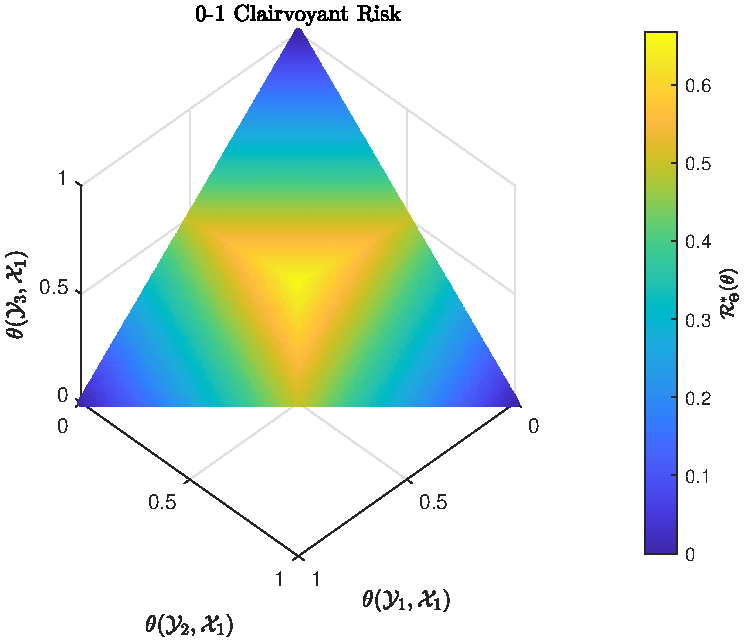
\includegraphics[width=0.8\linewidth]{Risk_clv_01.pdf}
%\caption{}
\label{fig:Risk_clv_01}
\end{figure}

\end{column}

\end{columns}
\vspace{1em}
\centering
\fcolorbox{NRL_blue}{NRL_blue}{\color{white}
\parbox{37em}{
\centering
\large
\textbf{Clairvoyant Risk $=$ Lower Bound for Conditional Risk}
}
}

\end{frame}



\begin{frame}
\frametitle{Bayesian Inference}

\large
\begin{equation*} 
\Downarrow \quad \Downarrow \quad \textbf{\textit{Model Unknown. Select Prior }} \bm{\mathrm{p}_\uptheta} \quad \Downarrow \quad \Downarrow 
\end{equation*}
\normalsize
\begin{IEEEeqnarray*}{rCl} \label{eq:risk}
\Rcal(f) & = & \Erm_{\uptheta}\big[ \Rcal_{\Theta}(f ; \uptheta) \big] = 1 - \Erm_{\xrm,\nbarrm}\Big[ \Prm_{\yrm | \xrm,\nbarrm} \big( f(\xrm;\nbarrm) \big) \Big]
\end{IEEEeqnarray*}

\vspace{-0.5em}
\hrulefill
\vspace{0.5em}

\begin{columns}[c]

\begin{column}{.5\linewidth}

\textbf{Optimal classifier}: Bayesian MAP
\begin{IEEEeqnarray*}{rCl} \label{eq:f_opt_xD}
f^*(\xrm;\nbarrm) & = & \argmax_{y \in \Ycal} \Prm_{\yrm | \xrm,\nbarrm}( y | \xrm,\nbarrm)
\end{IEEEeqnarray*}

\textbf{Minimum Bayes Probability of Error}:
\begin{equation*} \label{eq:risk_min}
\Rcal(f^*) = 1 - \Erm_{\xrm,\nbarrm} \left[ \max_{y \in \Ycal} \Prm_{\yrm | \xrm,\nbarrm}\big( y | \xrm,\nbarrm \big) \right]
\end{equation*}

\end{column}

\begin{column}{.5\linewidth}

\begin{block}{Predictive Distributions}

Bayesian PMF is the conditional expectation of the true PMF $\Prm_{\yrm | \xrm,\uptheta} \equiv \tilde{\uptheta}(\xrm)$:
\begin{equation*}
\Prm_{\yrm | \xrm,\nbarrm} = \Erm_{\uptheta | \xrm,\nbarrm}\big[ \Prm_{\yrm | \xrm,\uptheta} \big] \equiv \mu_{\tilde{\uptheta}(\xrm) | \xrm,\nbarrm}
\end{equation*}


\end{block}

\end{column}

\end{columns}


\end{frame}









\section{Distributions: Prior to Predictive}



\begin{frame}
\frametitle{Dirichlet Prior PDF}

\begin{columns}[c]

\begin{column}{.45\linewidth}

The probability density function (PDF) for the model random process $\uptheta \in \Theta$ is Dirichlet with parameters $\alpha(\cdot,\cdot) = 1$:
\begin{IEEEeqnarray*}{L}
\prm_{\uptheta}(\theta) = \Dir\big( \theta ; \alpha \big) \Big|_{\alpha(\cdot,\cdot) = 1} \\
\quad = \bigg[ \beta(\alpha)^{-1} \prod_{y \in \Ycal} \prod_{x \in \Xcal} \theta(y,x)^{\alpha(y,x) - 1} \bigg]_{\alpha(\cdot,\cdot) = 1} \\
\quad = \big( |\Ycal||\Xcal|-1 \big)!  
\end{IEEEeqnarray*}

\end{column}

\hspace{2ex}
\huge
\begin{column}{.1\linewidth}
$\Rightarrow$ \\ $\Rightarrow$
\end{column}
\normalsize
\hspace{-3ex}

\begin{column}{.45\linewidth}

Conditional PDF of $\tilde{\uptheta}$ given $\uptheta'$ is
\begin{IEEEeqnarray*}{L}
\prm_{\tilde{\uptheta} | \uptheta'}\big( \tilde{\theta} | \theta' \big) = \prm_{\tilde{\uptheta}}\big( \tilde{\theta} \big) \\
\quad= \prod_{x \in \Xcal} \Dir\Big( \tilde{\theta}(x) ; \alpha(\cdot,x) \Big) \Big|_{\alpha(\cdot,x) = 1} \\
\quad = \Big[ \big( |\Ycal|-1 \big)! \Big]^{|\Xcal|}
\end{IEEEeqnarray*}

\end{column}

\end{columns}

\vspace{1em}

\vspace{1em}
\centering
\fcolorbox{NRL_blue}{NRL_blue}{\color{white}
\parbox{37em}{
\centering
\large
\textbf{True predictive distribution $\tilde{\uptheta}$ is independent \\of the marginal model and inherits a uniform PDF}
}
}
\end{frame}








\begin{frame}
\frametitle{Model Posterior PDF}
\framesubtitle{Closed-Form}

\begin{itemize}
\item Independence of $\tilde{\uptheta}$ from $\uptheta'$ implies conditional independence of $\tilde{\uptheta}$ from $\xrm$ given $\nbarrm$
\item As the data PMF $\Prm_{\nbarrm | \uptheta}$ has exponential form, the Dirichlet PDF is a conjugate prior 

\end{itemize}
\vspace{0.5em}
\begin{IEEEeqnarray*}{rCl}
\prm_{\tilde{\uptheta} | \xrm,\nbarrm}\big( \tilde{\theta} | x,\bar{n} \big) & = & \prm_{\tilde{\uptheta} | \nbarrm}\big( \tilde{\theta} | \bar{n} \big) \\
& = & \prod_{x' \in \Xcal} \Dir\Big( \tilde{\theta}(x') ; \alpha(\cdot,x') \Big) \Big|_{\alpha(\cdot,x') = 1 + \bar{n}(\cdot,x')} \\
%= \prod_{x' \in \Xcal} \left[ \left( \sum_{y \in \Ycal} \bar{n}(y,x') + |\Ycal|-1 \right)! \prod_{y \in \Ycal} \frac{\tilde{\theta}(y,x')^{\bar{n}(y,x')}}{\big(\sum_{y \in \Ycal} \bar{n}(y,x')\big)!} \right] 
\end{IEEEeqnarray*}

\vspace{0.5em}

\centering
\fcolorbox{NRL_blue}{NRL_blue}{\color{white}
\parbox{37em}{
\centering
\large
\textbf{Posterior for model $\tilde{\uptheta}(x)$ is Dirichlet and dependent \\solely on the sufficient statistic elements $\nbarrm(\cdot,x)$}
}
}

\end{frame}



\begin{frame}
\frametitle{Model Posterior PDF}
\framesubtitle{Asymptotic Trend}

\begin{columns}[T]

\begin{column}{.6\linewidth}

\begin{itemize}
\item Covariance of Dirichlet $\prm_{\tilde{\uptheta}(x) | \nbarrm(\cdot,x)}$ decreases monotonically with concentration $\alpha'(x) \equiv \sum_{y \in \Ycal} \alpha(y,x)$
\item Localized around $\mu_{\tilde{\uptheta}(x) | \nbarrm(\cdot,x)} = \alpha(\cdot,x)/\alpha'(x)$
\end{itemize}
\Large
\begin{equation*} 
\Downarrow \quad \Downarrow
\end{equation*}
\normalsize
As $n'(x) \equiv \sum_{y \in \Ycal} \bar{n}(y,x) \to \infty$, the posteriors converge to 
\begin{IEEEeqnarray*}{L}
\prm_{\tilde{\uptheta}(x) | \nbarrm(\cdot,x)}\Big(\tilde{\theta}(x) | \bar{n}(\cdot,x) \Big) \to \delta\left( \tilde{\theta}(x) - \frac{\bar{n}(\cdot,x)}{n'(x)} \right)
\end{IEEEeqnarray*}

\end{column}

\begin{column}{.4\linewidth}

\begin{figure}
\centering
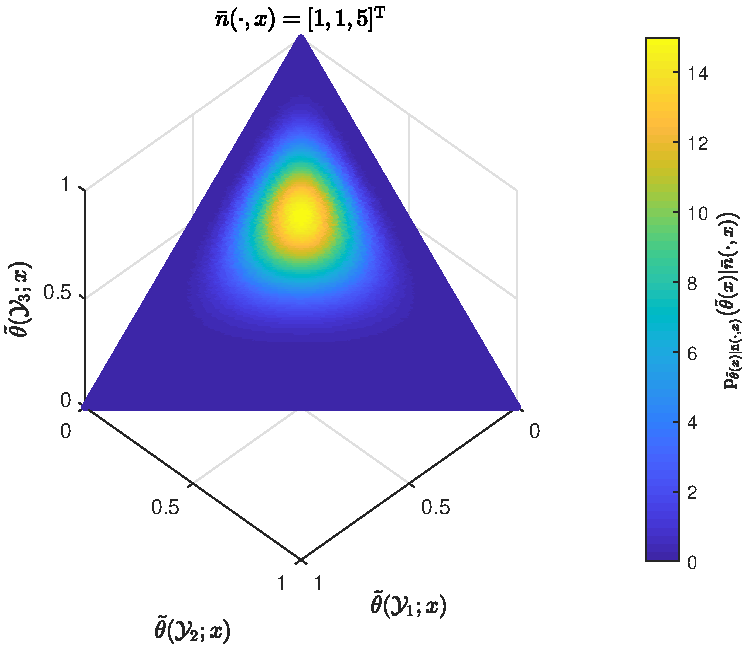
\includegraphics[width=0.9\linewidth]{P_theta_post_uni_tilde.pdf}
%\caption{}
\label{fig:P_theta_post_uni}
\end{figure}

\end{column}

\end{columns}

\vspace{1em}

\centering
\fcolorbox{NRL_blue}{NRL_blue}{\color{white}
\parbox{37em}{
\centering
\large
\textbf{Asymptotically consistent estimation of $\tilde{\uptheta}$ due to full support of prior}
}
}

\end{frame}




\begin{frame}
\frametitle{Bayesian Predictive PMF}

\textit{The Bayesian predictive PMF is a convex combination of two conditional distributions}:
\vspace{0.5em}
\begin{IEEEeqnarray*}{rCl} \label{P_y_xD_uniform}
\Prm_{\yrm | \xrm,\nbarrm}(\cdot | x,\bar{n}) & = & \mu_{\tilde{\uptheta}(x) | \nbarrm(\cdot,x)}\big( \bar{n}(\cdot,x) \big) \\
& \equiv & \left( \frac{|\Ycal|}{n'(x) + |\Ycal|} \right) \frac{1}{|\Ycal|} + \left( \frac{n'(x)}{n'(x) + |\Ycal|} \right) \frac{\bar{n}(\cdot,x)}{n'(x)} 
\end{IEEEeqnarray*}

\vspace{0.5em}

\begin{description}
\item[Prior Mean] Uniform PMF $\mu_{\tilde{\uptheta}(x)} = |\Ycal|^{-1}$ dependent only on the Dirichlet parameterization
\item[Conditional Empirical PMF] $\bar{n}(\cdot,x) / n'(x)$ dependent only on training data
\end{description}

\vspace{1em}

\centering
\fcolorbox{NRL_blue}{NRL_blue}{\color{white}
\parbox{37em}{
\centering
\large
\textbf{As the number of training data $n'(x)$ increases relative to the number of classes $|\Ycal|$, the predictive distribution tends toward the empirical PMF}
}
}

\end{frame}





\section{Bayesian Classifier and Error Trends}


\begin{frame}
\frametitle{Bayesian Classifier and Risk}

\textbf{Optimal Hypothesis}: the \emph{conditional majority decision}
\begin{IEEEeqnarray}{rCl} 
f^*(x;\bar{n}) & = & \argmax_{y \in \Ycal} \Prm_{\yrm | \xrm,\nbarrm}\big( y | x,\bar{n} \big) = \argmax_{y \in \Ycal} \bar{n}(y,x) \nonumber
\end{IEEEeqnarray}

\hrulefill
\vspace{0.5em}

\textbf{Minimum Expected Probability of Error}:
\begin{IEEEeqnarray*}{L}
\Rcal^* = 1 - \Erm_{\xrm,\Drm} \left[ \max_{y \in \Ycal} \Prm_{\yrm | \xrm,\Drm}(y | \xrm,\Drm) \right] = 1 - \sum_{x \in \Xcal} \frac{\Erm_{\nbarrm} \big[ \max_{y \in \Ycal} \bar{\nrm}(y,x) \big] + 1}{|\Ycal||\Xcal| + N} \nonumber \\
= 1 - \frac{\sum_{m=1}^{|\Ycal|} \binom{|\Ycal|}{m} (-1)^{m-1} \sum_{n=0}^{\big\lfloor\frac{N}{m}\big\rfloor} \prod_{l=1}^{|\Ycal||\Xcal|-1} \Big( 1-\frac{mn}{N+l} \Big)}{|\Ycal| + N/|\Xcal|} 
\end{IEEEeqnarray*}
\vspace{0.5em}
\begin{itemize}
\item[$*$] \emph{Efficient formula derived using Inclusion-Exclusion principle}
\end{itemize}

\end{frame}


\begin{frame}
\frametitle{Probability of Error Trends}
\framesubtitle{with Class/Data Set Sizes}

\begin{columns}[c]

\begin{column}{.5\linewidth}

\begin{figure}
\centering
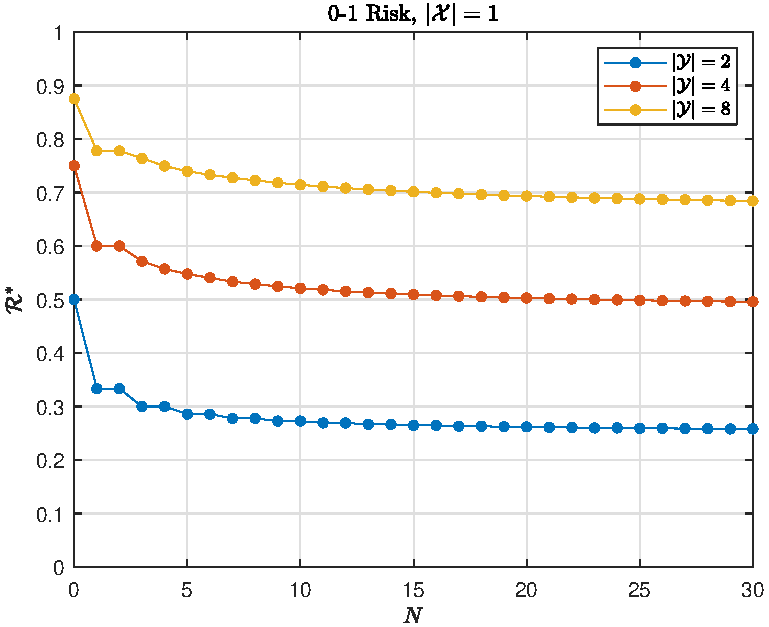
\includegraphics[width=0.8\linewidth]{Risk_01_uni_N_leg_My.pdf}
%\caption{Minimum 0--1 Risk for different numbers of classes}
\label{fig:Risk_01_uni_N_leg_My}
\end{figure}

\end{column}

\begin{column}{.5\linewidth}

\begin{figure}
\centering
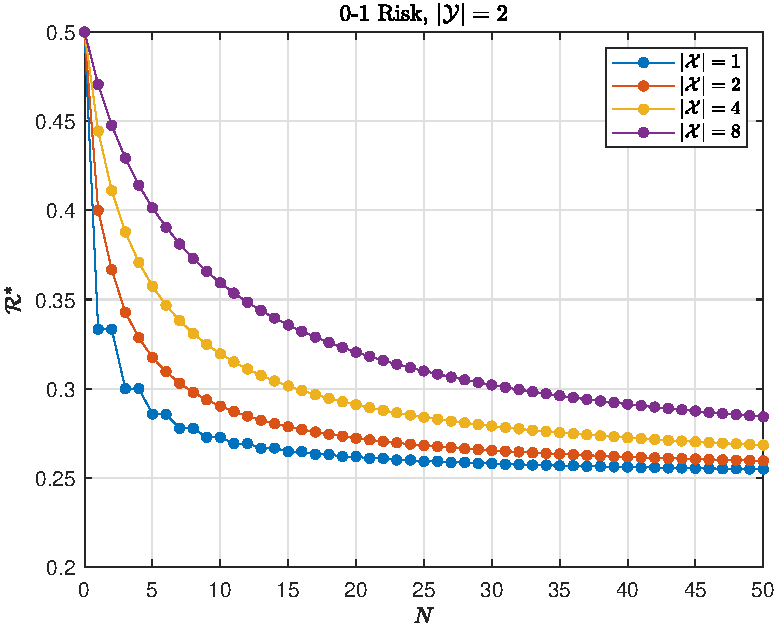
\includegraphics[width=0.8\linewidth]{Risk_01_uni_N_leg_Mx.pdf}
%\caption{Minimum 0--1 Risk for different numbers of possible observations}
\label{fig:Risk_01_uni_N_leg_Mx}
\end{figure}

\end{column}

\end{columns}

\begin{itemize}
\item Larger class sets $\Ycal$ raise the lower bound on probability of error
\item Larger observation set $\Xcal$ $\longrightarrow$ more data $N$ required to achieve the same level of performance
\end{itemize}

\end{frame}




\begin{frame}
\frametitle{Probability of Error Trends}
\framesubtitle{with Training Data Volume}

\begin{columns}[c]

\begin{column}{.5\linewidth}

\begin{itemize}
\item For binary classification, infinite training data only reduces the expected probability of error from 0.5 to 0.25
\item As $|\Ycal|$ increases, the probability of error tends to unity and any improvement due to training data becomes negligible
\end{itemize}

\begin{table}
\renewcommand{\arraystretch}{1.3}
\begin{tabular}{| c | c |}
\hline 
$N$ & $\Rcal^*$ \\
\hhline{|=|=|}
$0$ & $1 - |\Ycal|^{-1}$  \\ 
\hline
$\to \infty$ & $1 - |\Ycal|^{-1} \sum_{m=1}^{|\Ycal|} m^{-1}$ \\
\hline
\end{tabular}
%\caption{}
\end{table}

\end{column}

\begin{column}{.5\linewidth}

\begin{figure}
\centering
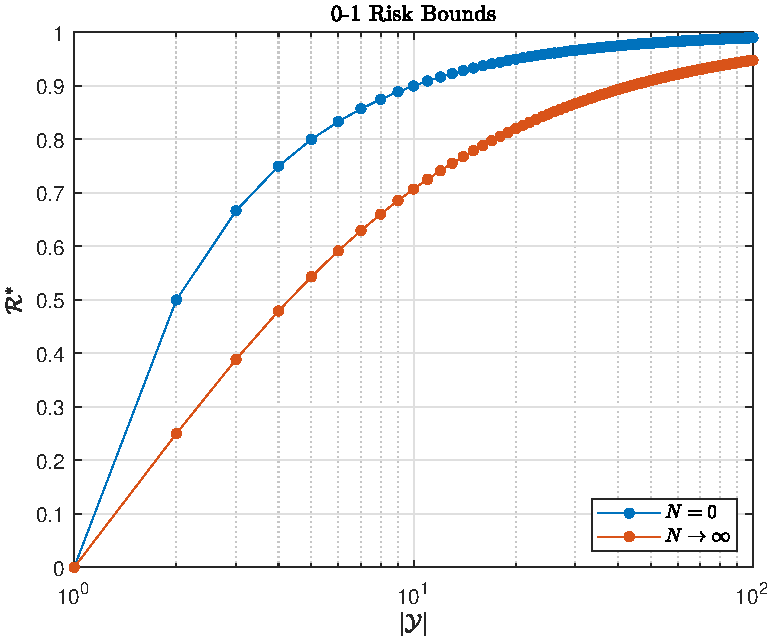
\includegraphics[width=1\linewidth]{Risk_01_uni_N_bounds.pdf}
%\caption{Minimum 0--1 Risk for zero and infinite number of training data}
\label{fig:Risk_01_uni_N_bounds}
\end{figure}

\end{column}

\end{columns}

\end{frame}


\begin{frame}
\frametitle{Comparison to Informative Classifiers}
\framesubtitle{Bayes Risk}

Classifiers derived from informative Dirichlet priors with $\alpha_f'(x) \gg |\Ycal||\Xcal|$ prioritize the prior mean $\mu_{\tilde{\uptheta}} = \alpha_f(\cdot,x) / \alpha_f'(x)$ for prediction

\vspace{-0.5em}
\begin{columns}[T]

\begin{column}{.5\linewidth}

\begin{figure}
\centering
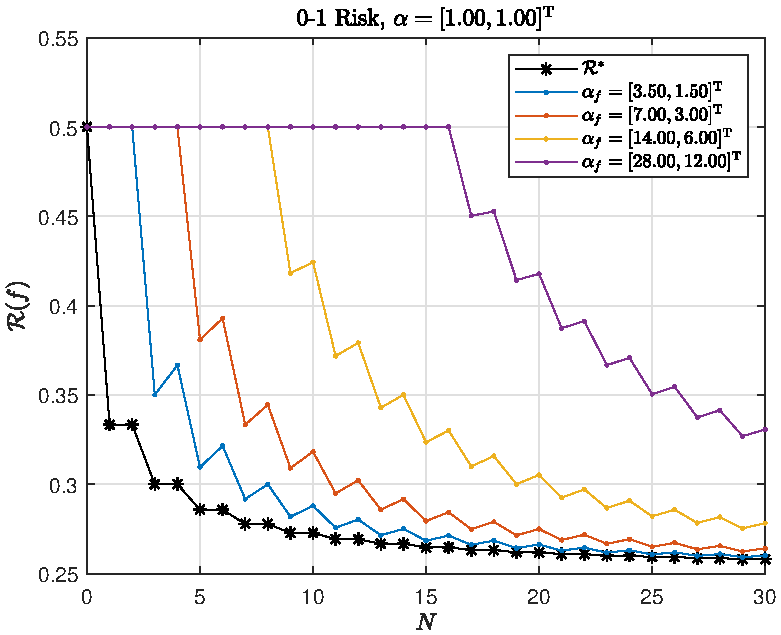
\includegraphics[width=0.8\linewidth]{Risk_01_Dir_N_leg_f_a0.pdf}
%\caption{}
\label{fig:Risk_01_Dir_N_leg_f_a0}
\end{figure}
\vspace{-2.5em}
\centering
\footnotesize
%Various $\alpha'(x)$

\end{column}

\begin{column}{.5\linewidth}

\begin{figure}
\centering
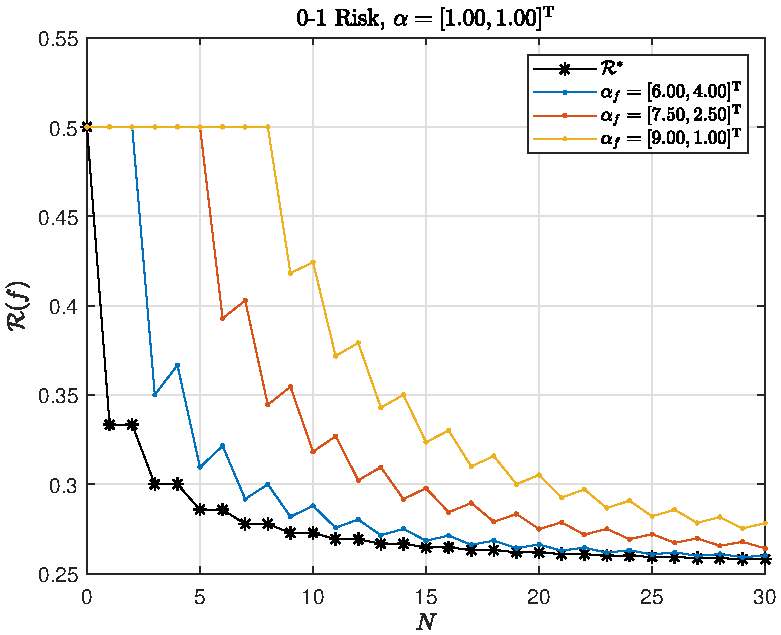
\includegraphics[width=0.8\linewidth]{Risk_01_Dir_N_leg_f_mu.pdf}
%\caption{}
\label{fig:Risk_01_Dir_N_leg_f_mu}
\end{figure}
\vspace{-2.5em}
\centering
\footnotesize
%Various $\mu_{\tilde{\uptheta}}$

\end{column}

\end{columns}

\vspace{1.8em}
\centering
\fcolorbox{NRL_blue}{NRL_blue}{\color{white}
\parbox{37em}{
\centering
\large
\textbf{Slower adaptation $\Rightarrow$ Higher Bayes probability of error}
}
}

\end{frame}



\begin{frame}
\frametitle{Comparison to Informative Classifiers}
\framesubtitle{Excess Conditional Risk}

\vspace{-1em}
\begin{columns}[c]

\begin{column}{.5\linewidth}

\begin{figure}
\centering
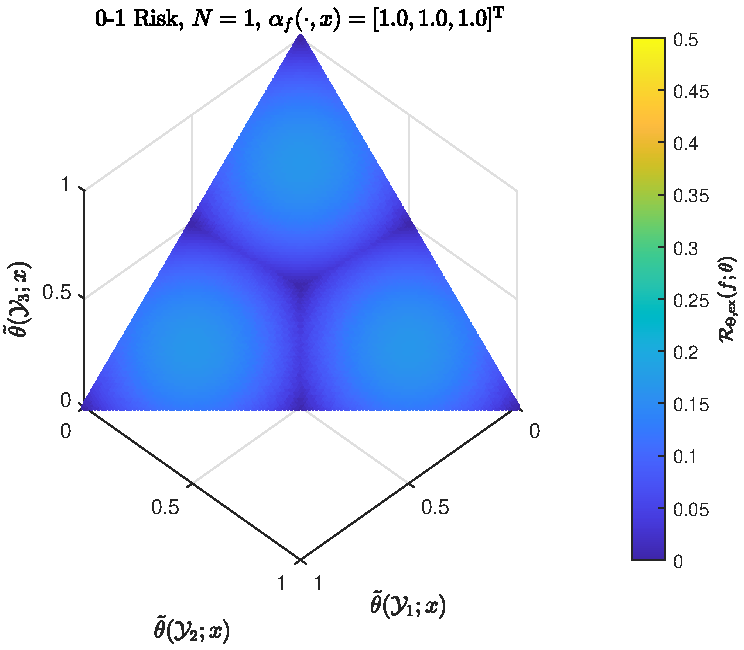
\includegraphics[width=0.8\linewidth]{Risk_cond_ex_01_Dir_theta__uni_clim.pdf}
%\caption{}
\label{fig:Risk_cond_ex_01_Dir_theta__uni}
\end{figure}

\end{column}

\begin{column}{.5\linewidth}

\begin{figure}
\centering
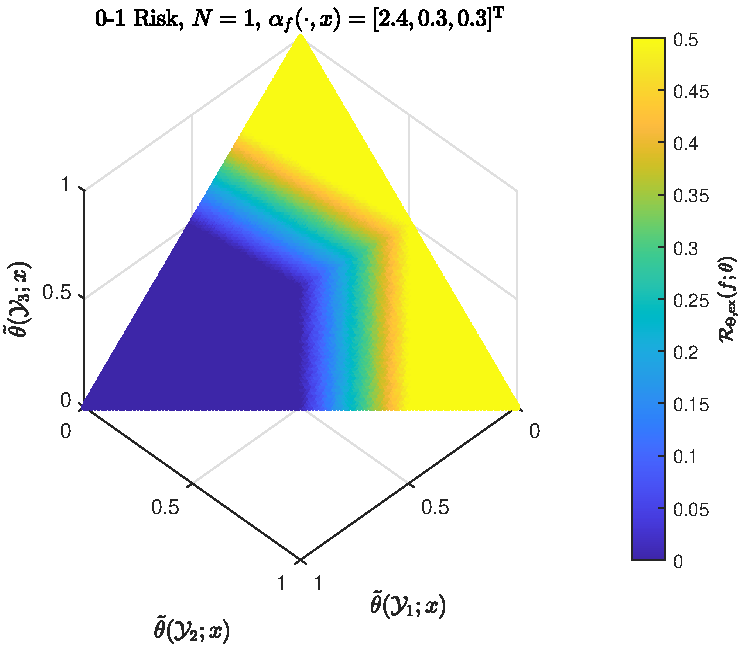
\includegraphics[width=0.8\linewidth]{Risk_cond_ex_01_Dir_theta__subj_clim.pdf}
%\caption{}
\label{fig:Risk_cond_ex_01_Dir_theta__subj}
\end{figure}

\end{column}

\end{columns}

\vspace{-0.2em}
\begin{block}{Trade-Off}
\textbf{Uniform prior provides a robust classifier for all unknown models $\theta$, limiting the space of high error models. However, fewer models achieve the clairvoyant risk.}
\end{block}


\end{frame}




\begin{frame}
\frametitle{Conclusions}

\begin{itemize}
\item The majority decision classifier designed with a uniform Dirichlet prior minimizes the possibility of maximal error for applications where the data distribution can not be adequately modeled
\item Full support of Dirichlet priors guarantees minimal risk in the limit of training data volume
\item Efficient closed-form for Bayesian probability of error provides a lower-bound for general classifiers
\end{itemize}

\begin{columns}[T]

\begin{column}{.55\linewidth}

\begin{itemize}
\item Low localization Dirichlet priors result in the same classifier - these priors are sensible for recognition applications where humans perform with low-error
\end{itemize}

\end{column}

\begin{column}{.4\linewidth}

\vspace{-2em}
\begin{figure}
\centering
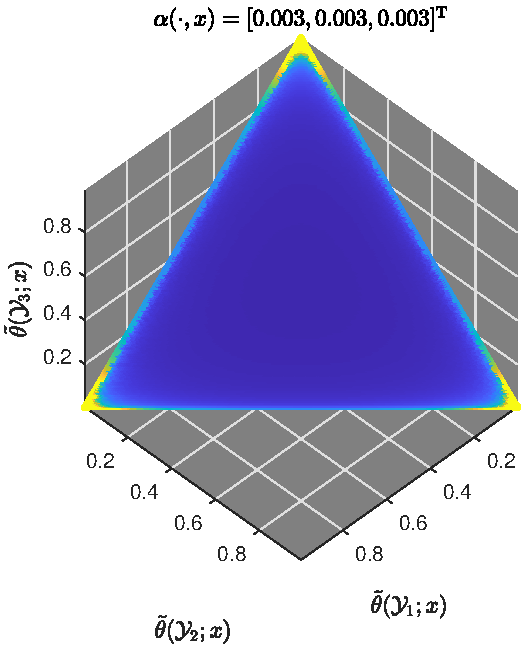
\includegraphics[width=0.5\linewidth]{P_theta_highVar.pdf}
%\caption{}
\label{fig:P_theta_highVar}
\end{figure}

\end{column}

\end{columns}


\end{frame}







\end{document}
